\documentclass[../mathNotesPreamble]{subfiles}

\providecommand{\relscalefact}{1.4}
\begin{document}
\relscale{\relscalefact}
  \section{2.2: Graphs of Linear Functions}
  %graph based on points
  %graph based on slope-int form
  %graph based on transformations

    \begin{defn*}[Parallel and Perpendicular lines]
      Let $L_1$ and $L_2$ be lines with slopes $m_1$ and $m_2$ respectively. If $L_1$ and $L_2$ are \emph{parallel}, then
        \[m_1=m_2.\]
      If $L_1$ and $L_2$ are \emph{perpendicular}, then
        \[m_1=-\frac{1}{m_2}.\]
    \end{defn*}
    
    \begin{ex*}\mbox{}
      \begin{extasks}[after-item-skip=\stretch{1}](1)
        \task Find the line \emph{parallel} to $y=\frac{3}{2}x+1$ that passes through the point $(-4,10)$.
        \task Find the line \emph{perpendicular} to $y=\frac{3}{2}x+1$ that passes through the point $(-3,4)$.
      \end{extasks}
    \end{ex*}
    \vspace*{\stretch{1}}
    \pagebreak

    \begin{defn*}
      The point(s) where a graph intersects the axes are called intercepts. 
      
      The \textbf{$x$-intercepts} are the points where a function intersects the $x$-axis.
      
      The \textbf{$y$-intercept} is the point where a function intersects the $y$-axis.
    \end{defn*}
    \begin{tasks}[label=\textbullet](2)
      \task To solve for the $y$-intercept:
        \begin{itemize}
          \item Set $x=0$,
          \item Solve for $y$.
        \end{itemize}
      \task To solve for the $x$-intercept:
        \begin{itemize}
          \item Set $y=0$,
          \item Solve for $x$.
        \end{itemize}
    \end{tasks}
    \begin{ex*}
      Find the $x$ and $y$ intercepts of the following:
      \begin{extasks}[after-item-skip=\stretch{1}](2)
        \task $y=\dfrac{4}{5}x-8$
        \task $3x+2y=18$
      \end{extasks}
      \vspace*{\stretch{1}}
    \end{ex*}
    \pagebreak

    \begin{ex*}
      Graph the following:
      \begin{extasks}[after-item-skip=\stretch{1}](2)
        \task 
          $y=-\dfrac{3}{2}x+3$

          \begin{center}
            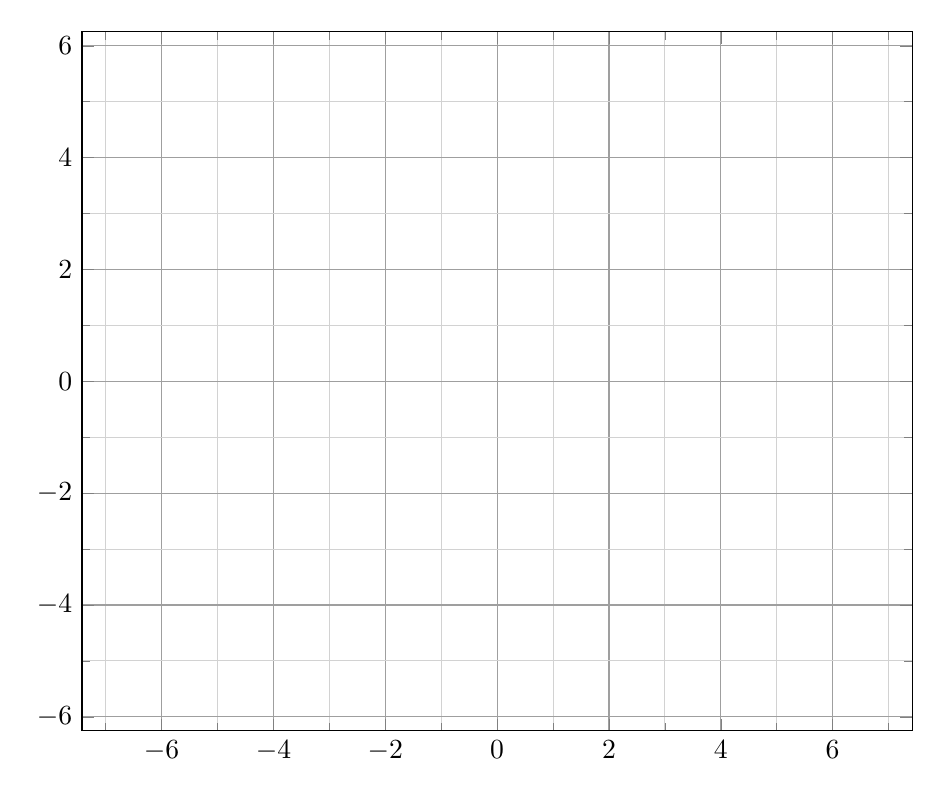
\begin{tikzpicture}
              \begin{axis}[
                  grid=both, %major,minor
                  grid style={line width=0.375pt, draw=gray!75},
                  axis equal,
                  minor grid style={draw=gray!35},
                  xmin=-6, xmax=6,
                  ymin=-6.25, ymax=6.25,
                  width=\linewidth,
                  minor x tick num=1,
                  minor y tick num=1,
                  xlabel=, ylabel=,
                  xtick={-8,-6,...,8},
                  ytick={-8,-6,...,8}
                  ]
              \end{axis}
            \end{tikzpicture}
          \end{center}
        \task 
          The line through $(-4,2)$ and $(1,4)$

          \begin{center}
            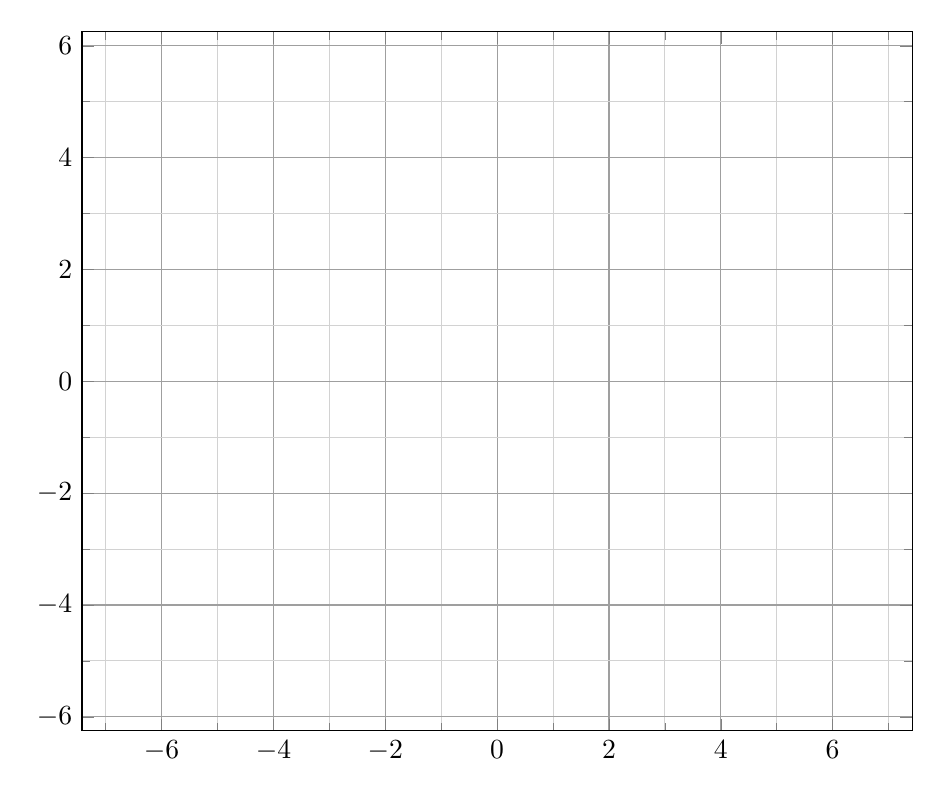
\begin{tikzpicture}
              \begin{axis}[
                  grid=both, %major,minor
                  grid style={line width=0.375pt, draw=gray!75},
                  axis equal,
                  minor grid style={draw=gray!35},
                  xmin=-6, xmax=6,
                  ymin=-6.25, ymax=6.25,
                  width=\linewidth,
                  minor x tick num=1,
                  minor y tick num=1,
                  xlabel=, ylabel=,
                  xtick={-8,-6,...,8},
                  ytick={-8,-6,...,8}
                  ]
              \end{axis}
            \end{tikzpicture}
          \end{center}
        \task 
          The horizontal line through $(2,3)$

          \begin{center}
            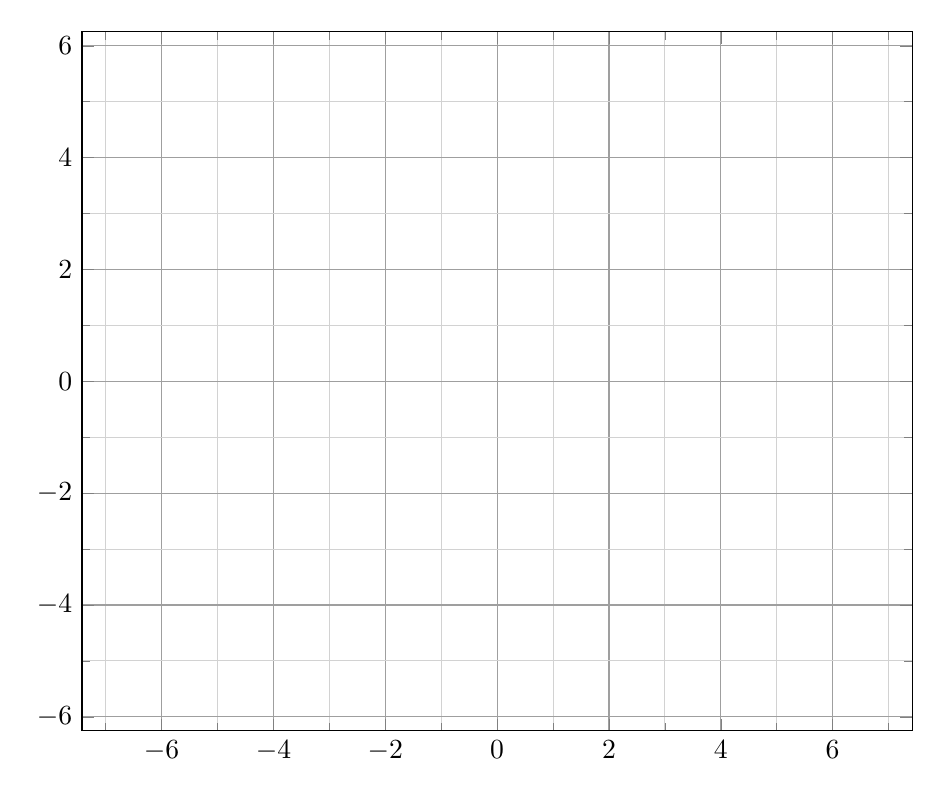
\begin{tikzpicture}
              \begin{axis}[
                  grid=both, %major,minor
                  grid style={line width=0.375pt, draw=gray!75},
                  axis equal,
                  minor grid style={draw=gray!35},
                  xmin=-6, xmax=6,
                  ymin=-6.25, ymax=6.25,
                  width=\linewidth,
                  minor x tick num=1,
                  minor y tick num=1,
                  xlabel=, ylabel=,
                  xtick={-8,-6,...,8},
                  ytick={-8,-6,...,8}
                  ]
              \end{axis}
            \end{tikzpicture}
          \end{center}
        \task 
          The vertical line through $(-1,5)$

          \begin{center}
            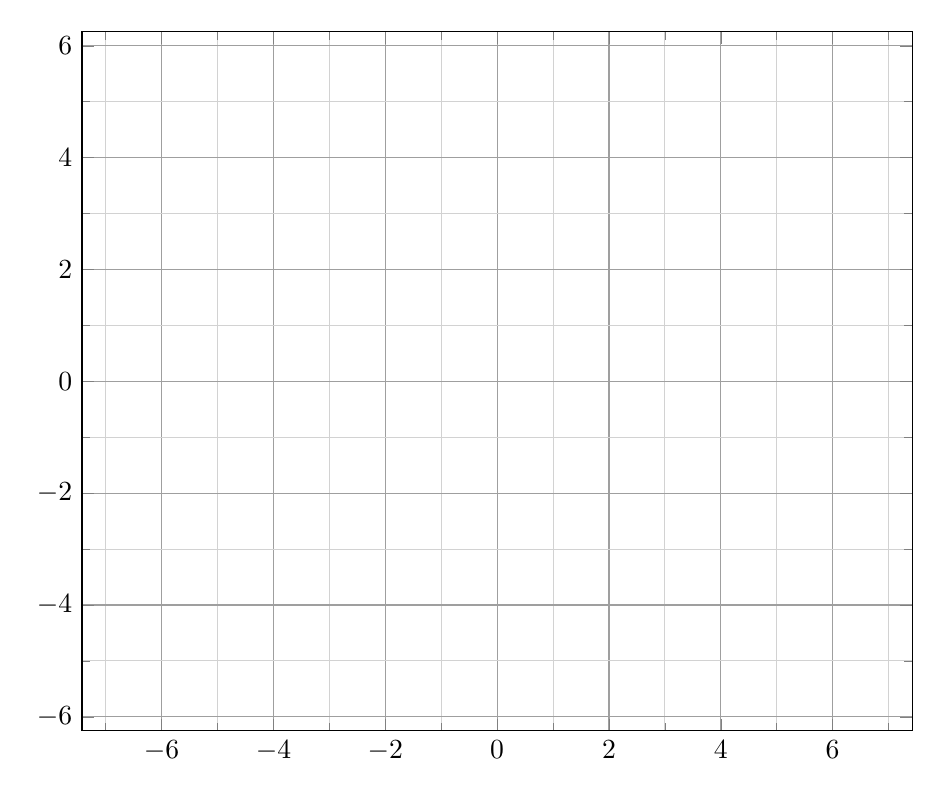
\begin{tikzpicture}
              \begin{axis}[
                  grid=both, %major,minor
                  grid style={line width=0.375pt, draw=gray!75},
                  axis equal,
                  minor grid style={draw=gray!35},
                  xmin=-6, xmax=6,
                  ymin=-6.25, ymax=6.25,
                  width=\linewidth,
                  minor x tick num=1,
                  minor y tick num=1,
                  xlabel=, ylabel=,
                  xtick={-8,-6,...,8},
                  ytick={-8,-6,...,8}
                  ]
              \end{axis}
            \end{tikzpicture}
          \end{center}
      \end{extasks}
      \vspace*{\stretch{1}}
    \end{ex*}

      \begin{extasks}[after-item-skip=\stretch{1}](2)
        \task 
          $8x-10y=40$

          \begin{center}
            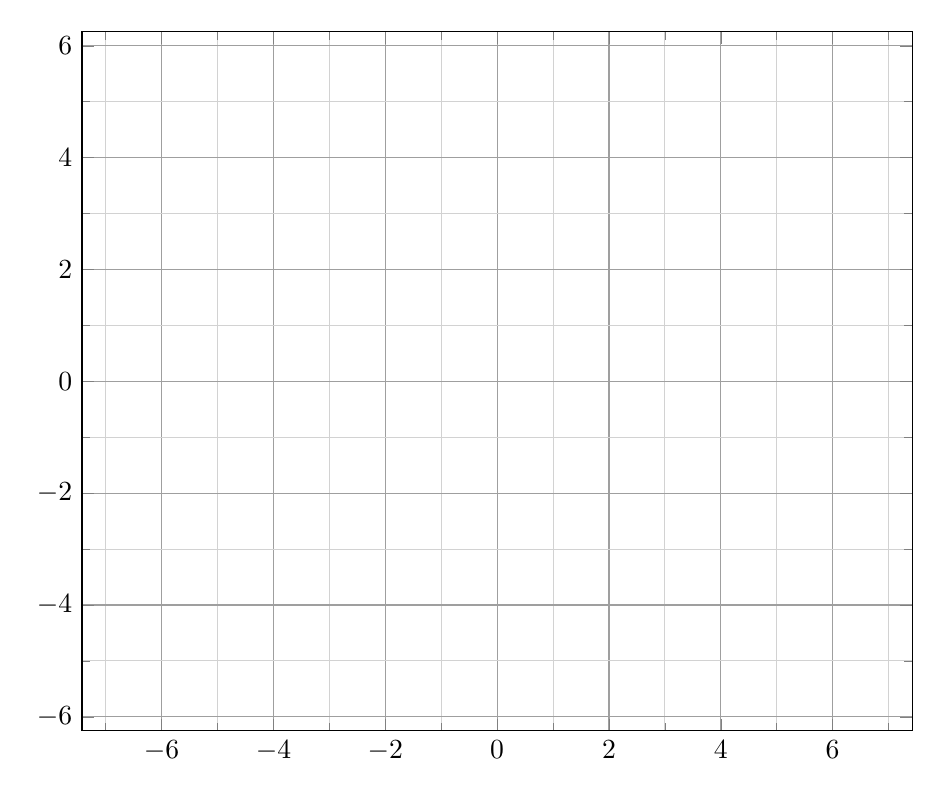
\begin{tikzpicture}
              \begin{axis}[
                  grid=both, %major,minor
                  grid style={line width=0.375pt, draw=gray!75},
                  axis equal,
                  minor grid style={draw=gray!35},
                  xmin=-6, xmax=6,
                  ymin=-6.25, ymax=6.25,
                  width=\linewidth,
                  minor x tick num=1,
                  minor y tick num=1,
                  xlabel=, ylabel=,
                  xtick={-8,-6,...,8},
                  ytick={-8,-6,...,8}
                  ]
              \end{axis}
            \end{tikzpicture}
          \end{center}
        \task 
          $y=-4x-5$

          \begin{center}
            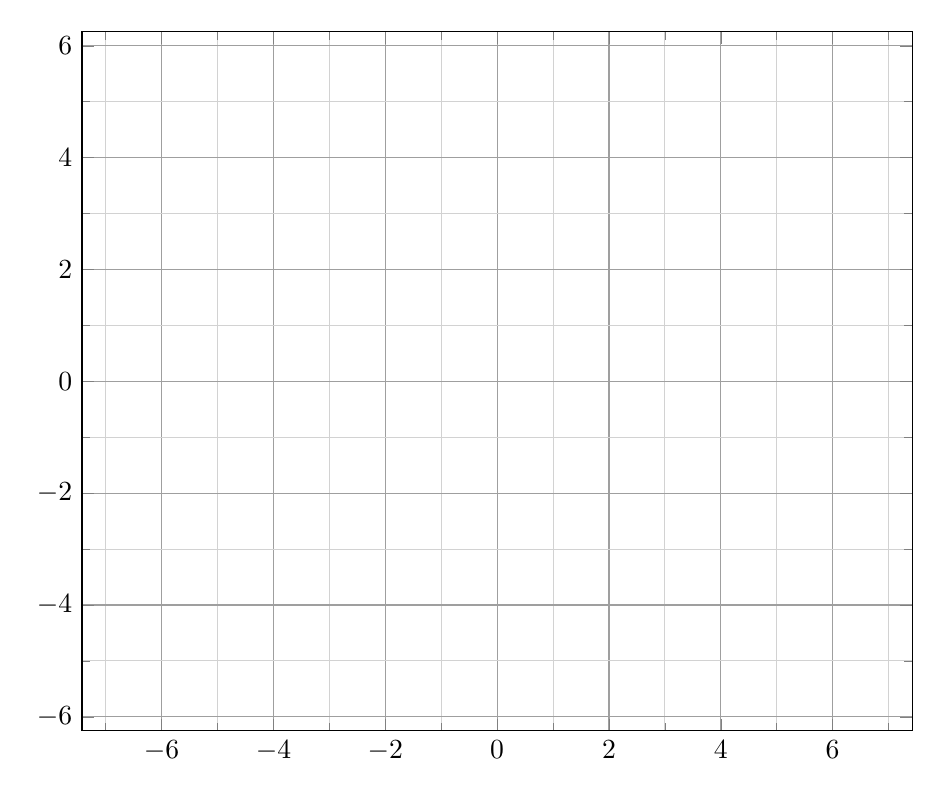
\begin{tikzpicture}
              \begin{axis}[
                  grid=both, %major,minor
                  grid style={line width=0.375pt, draw=gray!75},
                  axis equal,
                  minor grid style={draw=gray!35},
                  xmin=-6, xmax=6,
                  ymin=-6.25, ymax=6.25,
                  width=\linewidth,
                  minor x tick num=1,
                  minor y tick num=1,
                  xlabel=, ylabel=,
                  xtick={-8,-6,...,8},
                  ytick={-8,-6,...,8}
                  ]
              \end{axis}
            \end{tikzpicture}
          \end{center}
        \task 
          Through $(1,1)$, parallel to $y=2x-4$

          \begin{center}
            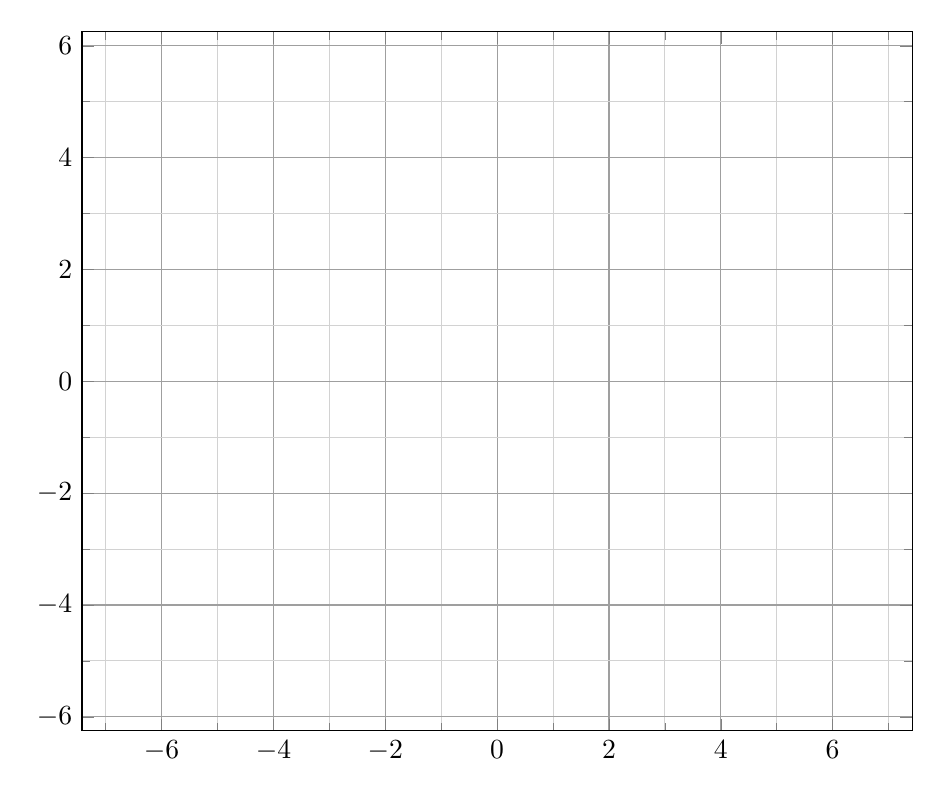
\begin{tikzpicture}
              \begin{axis}[
                  grid=both, %major,minor
                  grid style={line width=0.375pt, draw=gray!75},
                  axis equal,
                  minor grid style={draw=gray!35},
                  xmin=-6, xmax=6,
                  ymin=-6.25, ymax=6.25,
                  width=\linewidth,
                  minor x tick num=1,
                  minor y tick num=1,
                  xlabel=, ylabel=,
                  xtick={-8,-6,...,8},
                  ytick={-8,-6,...,8}
                  ]
              \end{axis}
            \end{tikzpicture}
          \end{center}
        \task 
          Through $(3,-2)$, perp. to $y=\dfrac{1}{3}x-1$

          \begin{center}
            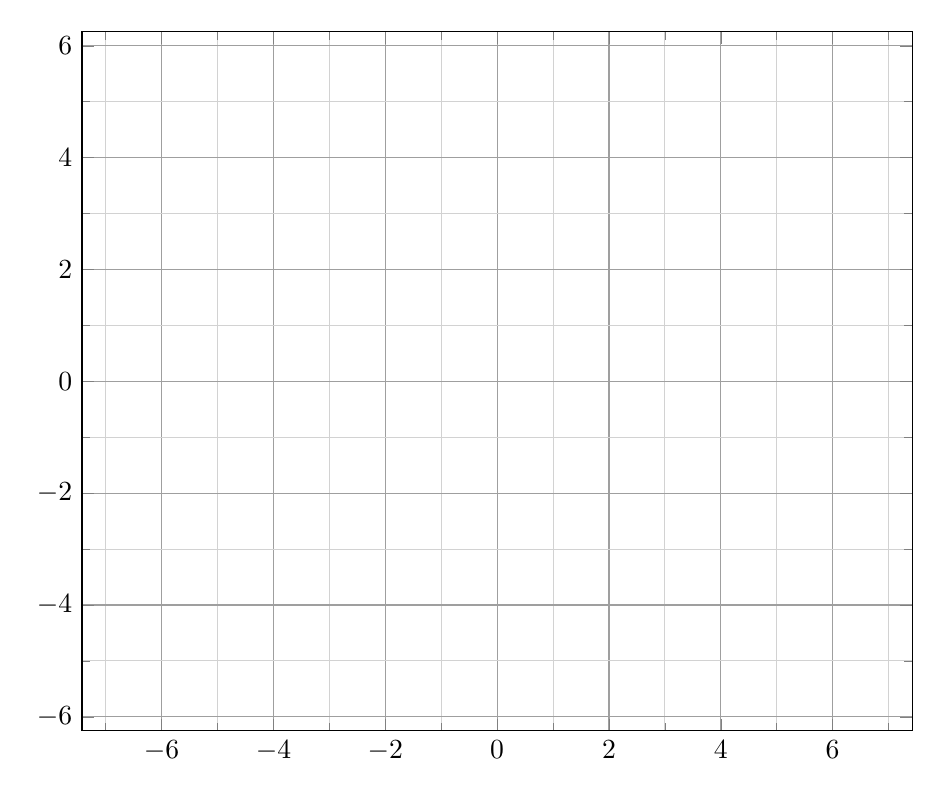
\begin{tikzpicture}
              \begin{axis}[
                  grid=both, %major,minor
                  grid style={line width=0.375pt, draw=gray!75},
                  axis equal,
                  minor grid style={draw=gray!35},
                  xmin=-6, xmax=6,
                  ymin=-6.25, ymax=6.25,
                  width=\linewidth,
                  minor x tick num=1,
                  minor y tick num=1,
                  xlabel=, ylabel=,
                  xtick={-8,-6,...,8},
                  ytick={-8,-6,...,8}
                  ]
              \end{axis}
            \end{tikzpicture}
          \end{center}
      \end{extasks}
    \pagebreak

  \pagebreak
\end{document}
